%%%%%%%%%%%%%%%%%%%%%%%%%%%%%%%%%%%%%%%%%%%%%%%%%%%%%%%%%%%%%%%%%%%%%%%%%%%
%% This file is part of the book
%%
%% Algorithmic Graph Theory
%% http://code.google.com/p/graph-theory-algorithms-book/
%%
%% Copyright (C) 2009, 2010 Minh Van Nguyen <nguyenminh2@gmail.com>
%%
%% See the file COPYING for copying conditions.
%%%%%%%%%%%%%%%%%%%%%%%%%%%%%%%%%%%%%%%%%%%%%%%%%%%%%%%%%%%%%%%%%%%%%%%%%%%

\subfigure[Binomial heap as a forest.]{
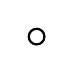
\begin{tikzpicture}
[-,thick,%
  every node/.style={shape=circle,inner sep=2pt,draw,thick}]
\node {};
\end{tikzpicture}
%%
%%
\qquad
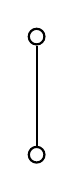
\begin{tikzpicture}
[-,thick,%
  every node/.style={shape=circle,inner sep=2pt,draw,thick}]
\node {}
  child {node {}};
\end{tikzpicture}
%%
%%
\qquad
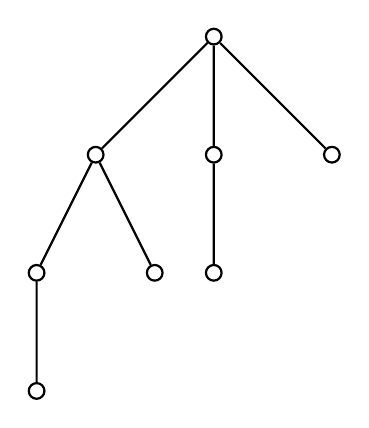
\begin{tikzpicture}
[-,thick,%
  every node/.style={shape=circle,inner sep=2pt,draw,thick}]
\node {}
  child {node {}
    child {node {}
      child {node {}}
    }
    child {node {}}
  }
  child {node {}
    child {node {}}
  }
  child {node {}};
\end{tikzpicture}
}
%%
%%
\qquad
\subfigure[Binomial heap as a tree.]{
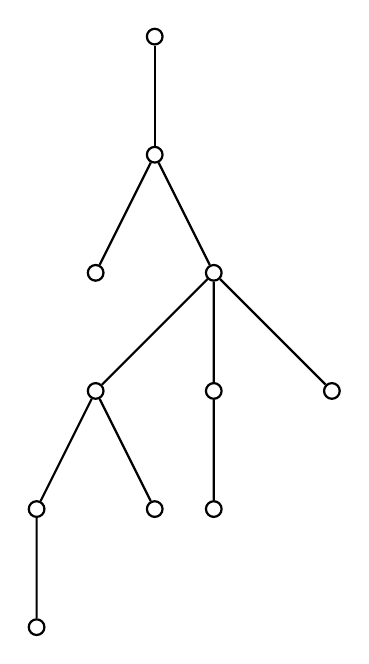
\begin{tikzpicture}
[-,thick,%
  every node/.style={shape=circle,inner sep=2pt,draw,thick}]
\node {}
  child {node {}
    child {node {}}
    child {node{}
      child {node {}
        child {node {}
          child {node {}}
        }
        child {node {}}
      }
      child {node {}
        child {node {}}
      }
      child {node {}}
    }
  };
\end{tikzpicture}
}
